\chapter{IMPLEMENTASI}
\tab Pada bab ini akan dipaparkan implementasi dari sistem yang telah dibangun. Bahasa pemrograman yang digunakan adalah bahasa pemrograman Arduino (\textit{Sketch}) yang menyerupai bahasa C untuk memprogram mikrokontroler dan Python untuk menghubungkan mikrokontroler dengan Bot Telegram sebagai pengendali mikrokontrolernya.

\section{Lingkungan Implementasi}
\tab Lingkungan implementasi dalam pembuatan sistem "EasyMeeting" meliputi perangkat keras dan perangkat lunak yang digunakan untuk mengimplementasikan sistem yang telah dirancang adalah sebagai berikut:
\begin{enumerate}
	\item Perangkat Keras
	\begin{itemize}
		\item Komponen Mikrokontroler
		\begin{itemize}
			\item NodeMCU
			\item DHT11
			\item \textit{Breadboard}
			\item Resistor
			\item \textit{Jumper Wires}
			\item LED \textit{Light Bulb}
			\item \textit{Infrared Sensor Module}
			\item \textit{Infrared Receiver Module}
		\end{itemize}
		\item Laptop
		\begin{itemize}
			\item \textit{Processor} Intel(R) Core(TM) i7-4510U CPU @ 2.00GHz
			\item Memori 4 GB (3,92514 GB)
		\end{itemize}
	\end{itemize}
	\item Perangkat Lunak
	\begin{itemize}
		\item Sistem Operasi Linux (Linux Mint 18.3 Sylvia)
		 64-bit
		\item \textit{Text Editor} Visual Studio Code
		\item Arduino \textit{Software} IDE
		\item Bahasa Pemrograman Python
		\item \textit{Version Control System} Git
	\end{itemize}
\end{enumerate}

\section{Implementasi Rangkaian Mikrokontroler}
\tab Pada bagian ini akan dijelaskan mengenai implementasi rangkaian mikrokontroler pada sistem EasyMeeting. Untuk pengimplementasiannya, dibutuhkan beberapa komponen mikrokontroler yaitu:
\begin{itemize}
	\item NodeMCU
	\item DHT11
	\item \textit{Breadboard}
	\item Resistor
	\item \textit{Jumper Wires}
	\item LED \textit{Light Bulb}
	\item \textit{Infrared Sensor Module}
	\item \textit{Infrared Receiver Module}
\end{itemize}
\tab Semua komponen di atas kemudian dirangkai menjadi satu kesatuan sesuai dengan perancangan sistem. Langkah-langkah yang dilakukan adalah:
\begin{enumerate}
	\item Menghubungka
\end{enumerate}

\section{Implementasi Lapisan Kontrol Sistem}
\tab Pada bagian ini akan dijelaskan mengenai lapisan kontrol sistem yang berfungsi untuk mengontrol keseluruhan sistem EasyMeeting, meliputi kontrol mikrokontroler hingga menghubungkan mikrokontroler dengan antarmuka pengguna (Bot API Telegram). Lapisan kontrol sistem dibuat menggunakan bahasa pemrograman Python.

\section{Implementasi Antarmuka Pengguna}
\tab Pada bagian ini akan dijelaskan mengenai bagaimana pengguna dapat berinteraksi dengan sistem EasyMeeting melalui platform Telegram. Telegram menyediakan dua jenis API yang dapat dikembangkan bebas oleh pengguna, yakni Telegram API dan Bot API. Penulis memanfaatkan Bot API Telegram untuk membuat antarmuka sistem berupa \textit{chat bot} yang dapat berinteraksi dengan pengguna.
\tab Langkah-langkah yang dilakukan untuk membuat

\subsection{Menyalakan Lampu dan AC Ruangan}

\subsection{Mematikan Lampu dan AC Ruangan}

\subsection{Melihat Status Kondisi Lampu dan AC Ruangan}

\subsection{Mengukur Suhu Ruangan}


\subsection{Tampilan Halaman Menambahkan \textit{Request} Relokasi}
Pada halaman menambahkan \textit{request} relokasi menggunakan HTML, CSS, PHP dan Javascript. Sebuah \textit{form} ditampilkan kemudian user mengisikan data-data yang diperlukan. \textit{Form} tersebut akan menampung data-data yang diperlukan, kemudian akan disimpan ke dalam basis data sistem. Gambar \ref{figure:tambahReqRelokasi} adalah tampilan dan gambar \ref{lst:addrelokasi1}, \ref{lst:addrelokasi2} dan \ref{lst:addrelokasi3} adalah potongan kode halaman menambahkan \textit{request} relokasi.
\begin{figure}[h!]
\centerline
{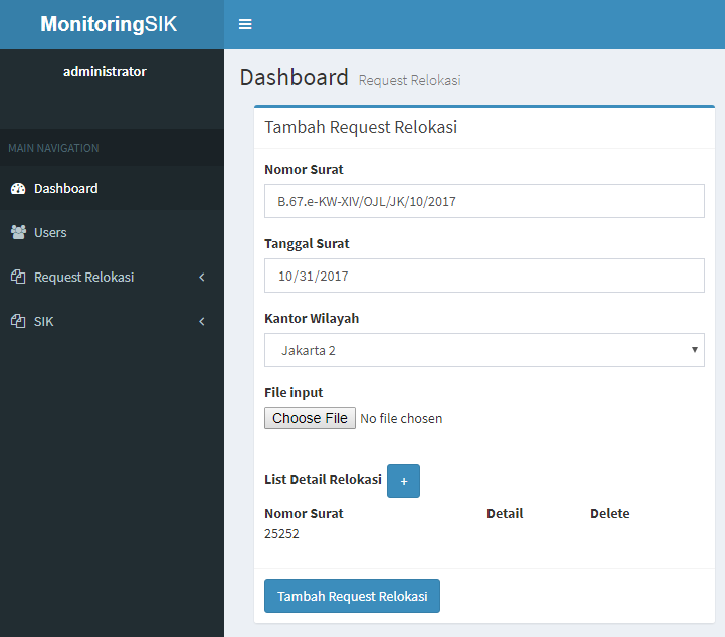
\includegraphics[width=10cm,height=7.5cm]{bab5/addReqRelokasi.png}}
\caption{Potongan Halaman Menambahkan \textit{Request} Relokasi}
\label{figure:tambahReqRelokasi}
\end{figure}

\lstinputlisting[language=PHP, firstline=34, lastline=45, firstnumber=1, caption=Potongan Kode Tampilan Menambahkan \textit{Request} Relokasi (1), label={lst:addrelokasi1}]{bab5/src/RelocationRequestController.php}
\lstinputlisting[language=PHP, firstline=46, lastline=82, firstnumber=14, caption=Potongan Kode Tampilan Menambahkan \textit{Request} Relokasi (2), label={lst:addrelokasi2}]{bab5/src/RelocationRequestController.php}
\lstinputlisting[language=PHP, firstline=83, lastline=109, firstnumber=51, caption=Potongan Kode Tampilan Menambahkan \textit{Request} Relokasi (3), label={lst:addrelokasi3}]{bab5/src/RelocationRequestController.php}

